\documentclass[slidestop,compress,mathserif]{beamer}
\usetheme{Aalborg}

\pgfdeclareimage[height=1cm]{mainlogo}{argolab}
\logo{\pgfuseimage{mainlogo}}

\pgfdeclareimage[height=1.5cm]{titlepagelogo}{argolab}
\titlegraphic{% is placed on the bottom of the title page
  \pgfuseimage{titlepagelogo}
%  \hspace{1cm}\pgfuseimage{titlepagelogo2}
}

\title{How does a BBS Work?}
\subtitle{Argo: For Example}
\author[wodesuck]
{ wodesuck\\ \href{mailto:wodesuck@gmail.com}{{\tt wodesuck@gmail.com}} }

\institute[ Argolab\\ Sun Yat-sen University ]
{ Argolab\\ Sun Yat-sen University }

\begin{document}

  {\aauwavesbg
  \begin{frame}[plain,noframenumbering]
    \titlepage
  \end{frame}}

  \section{Intro}
  \begin{frame}
    \frametitle{Question}
    \begin{block}{What should a BBS do?}
      \begin{itemize}
        \item response telnet requests
        \item response http requests
        \item deal with user information
        \item deal with board and topic
      \end{itemize}
    \end{block}
  \end{frame}

  \section{Telnet}
  \begin{frame}
    \frametitle{At the very beginning\dots}
    \pause
    \begin{block}{How to response telnet requests?}
      \begin{itemize}
        \item fork(): create a child process
        \item Each request handled by one process
      \end{itemize}
    \end{block}
    \pause
    \begin{block}{And how to communicate between processes?}
      \begin{itemize}
        \item Why commuincation needed: users can get the states of others
        \item shm: shared memory
      \end{itemize}
    \end{block}
    \pause
    \begin{block}{How to store the data?}
      \begin{itemize}
        \item Write C structures into file
      \end{itemize}
    \end{block}
  \end{frame}
  \begin{frame}
    \frametitle{Now we have a telnet server like this}
    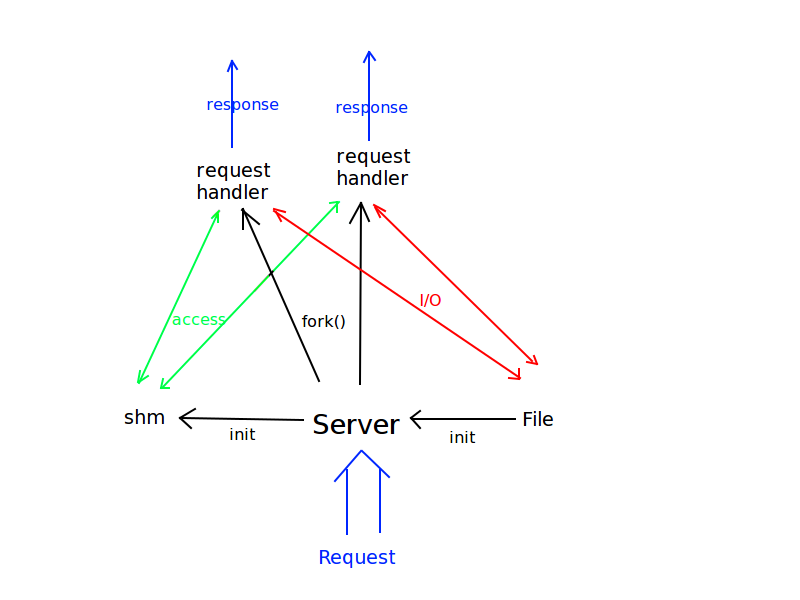
\includegraphics[scale=0.35]{telnet.png}
  \end{frame}

  \section{Web(the old version)}
  \begin{frame}
    \pause
    \frametitle{Then, we want a BBS on webpages}
    \begin{block}{websrc works similarly as telnet, except}
      \begin{itemize}
        \item handling http requests
        \item responsing html pages
      \end{itemize}
    \end{block}
    \pause
    \begin{block}{How to handle a http request}
      \begin{itemize}
        \item Routing table
      \end{itemize}
    \end{block}
  \end{frame}

  \section{The New Argo}
  \begin{frame}
    \frametitle{The New Argo}
    \begin{block}{Two parts}
      \begin{description}
        \item[jsbbs] the front-end, written by entire javascript
        \item[phpbbs] the back-end, only handles AJAX requests and responses JSON
      \end{description}
    \end{block}
    \begin{itemize}
      \item The front-end and back-end are completely independent
      \item phpbbs access BBS with a php extension in C
    \end{itemize}
  \end{frame}
  \begin{frame}
    \frametitle{The New Argo}
    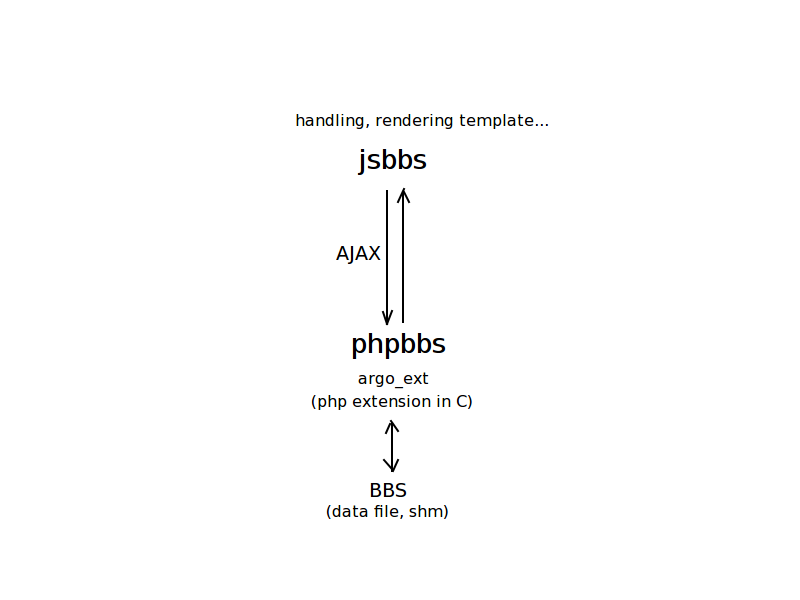
\includegraphics[scale=0.35]{newargo.png}
  \end{frame}

  \begin{frame}
    \frametitle{Working with Database}
    \pause
    \begin{block}{Using RDBMS, for}
      \begin{itemize}
        \item better flexibillity
        \item easier to migrate
      \end{itemize}
    \end{block}
    \pause
    \begin{block}{Compatibility with Existing Systems}
      \begin{itemize}
        \item phpbbs handing the database
        \item telnet and websrc send singals to phpbbs
      \end{itemize}
    \end{block}
  \end{frame}

  \begin{frame}
    \frametitle{Working with Database}
    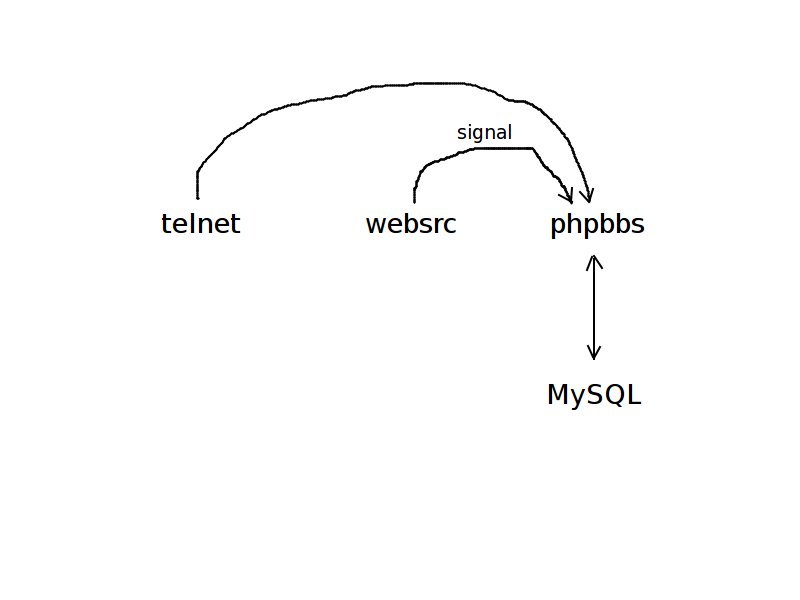
\includegraphics[scale=0.35]{withdb.png}
  \end{frame}

  {\aauwavesbg
  \begin{frame}[plain,noframenumbering]
    \finalpage{Thanks.}
  \end{frame}}

\end{document}
